La figura de este problema muestra dos cargas puntuales, $Q_1$ = 4.0 $\mu$C y $Q_2$ =-1.5 $\mu$C. Una carga positiva $q$ = 2.0 $\times$ 10$^{-7}$C, es colocada en el punto $P_1$ situado a 5.0 cm de $Q_2$. Suponiendo que estas cargas se encuentran en el aire, responda:
\begin{enumerate}
    \item ¿Cuál es la magnitud y el sentido de la fuerza ejercida por $Q_1$ sobre $q$?
    \item ¿Cuál es la magnitud y el sentido de la fuerza ejercida por $Q_2$ sobre $q$?
    \item ¿Cuál es la magnitud y el sentido de la fuerza eléctrica resultante que actúa sobre $q$?
\end{enumerate}
\begin{figure}[h!]
  \centering
  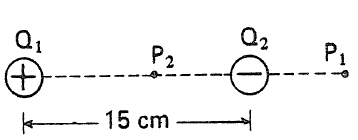
\includegraphics[scale=0.5]{figuras/fig_alvarenga_p825_14.png}
  \caption{Problema 27}
\end{figure}